\documentclass{beamer}
\usepackage[utf8]{inputenc}
\usepackage{graphicx}
\usepackage{svg}
\usetheme{Goettingen}

\title{Segurança em redes}
\subtitle{exemplos de exploits comuns e como lidar com elas}
\author{Giuliano Oliveira de Macedo}
\institute{}
\date{}

\begin{document}

\begin{frame}
\titlepage 
\end{frame}

\section{Importância de segurança em redes}

\begin{frame}
\frametitle{Modelo de software TCP/IP }
\begin{figure}[htp]
	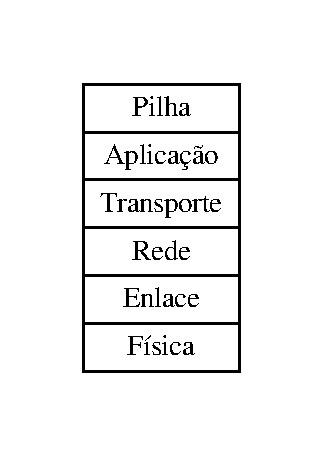
\includegraphics[width=6cm]{pilha1.pdf}
\end{figure}

\end{frame}

\begin{frame}
\frametitle{Modelo de software TCP/IP }
\begin{figure}[htp]
	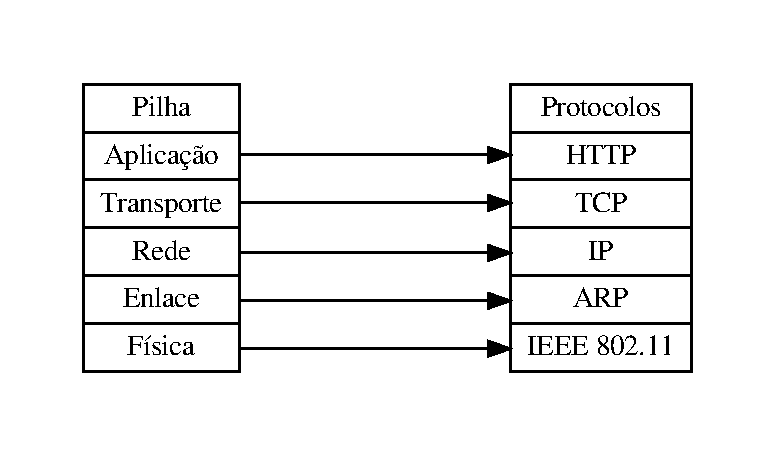
\includegraphics[width=10cm]{pilha2.pdf}
\end{figure}

\end{frame}

\begin{frame}
\frametitle{Modelo de software TCP/IP }
\begin{figure}[htp]
	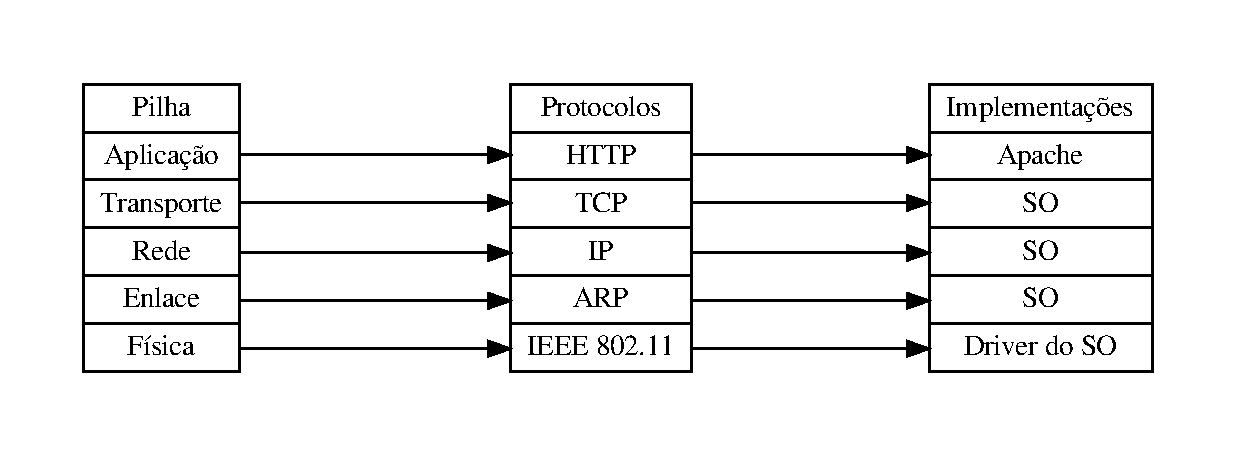
\includegraphics[width=10cm]{pilha3.pdf}
\end{figure}
\end{frame}

\section{Contextualização}
\begin{frame}
	\frametitle{Contextualização}
	\begin{itemize}
		\item CVE
		\begin{figure}[htp]
			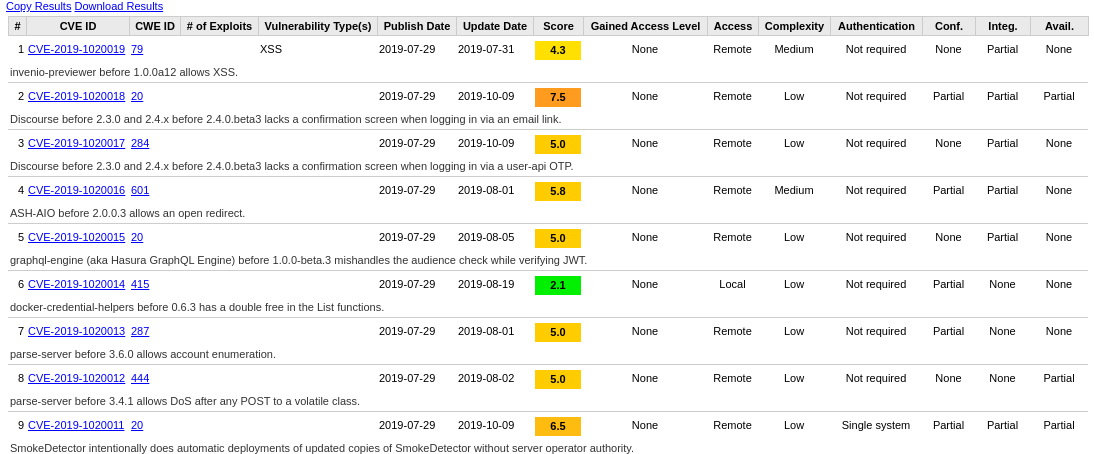
\includegraphics[width=9cm]{cve.png}
		\end{figure}
	\end{itemize}
\end{frame}

\begin{frame}
	\frametitle{Contextualização}
	\begin{itemize}
		\item Exploits
		\begin{itemize}
			\item Buffer overlfow
			\item DoS
			\item Execução de código
			\item Corrupção de Memória
			\item Sql Injection
			\item XSS
			\item Bypassing
			\item Ganhar informações
			\item Elevar previlégio
			\item etc
		\end{itemize}
	\end{itemize}
\end{frame}
\section{Ataques}
\begin{frame}
	\frametitle{Ataques}
	\begin{itemize}
		\item XSS (Cross server scripting)
		\item Heartbleed (Buffer overflow no protocolo TLS)
		\item ARP Spoofing (Manipulação de servidores/clientes ARP com o fim de espionagem)
	\end{itemize}
	\begin{figure}[htp]
		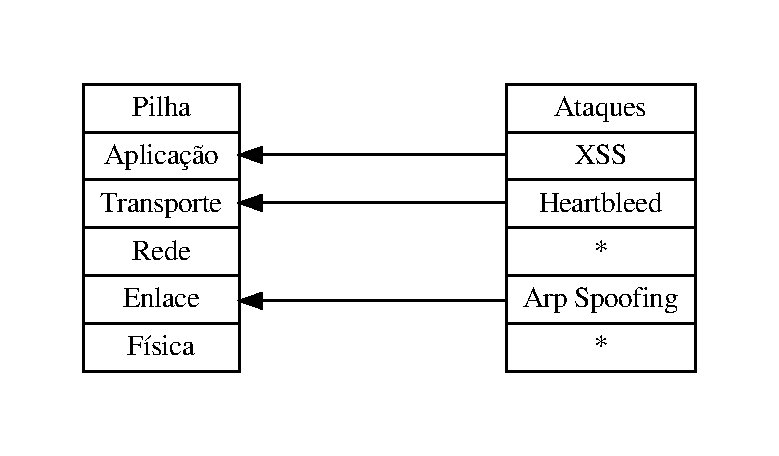
\includegraphics[width=8cm]{pilha_ataque.pdf}
	\end{figure}
\end{frame}

\subsection{XSS}
\begin{frame}
\frametitle{XSS}
\end{frame}

\subsection{Heartbleed}
\begin{frame}
\frametitle{Heartbleed}
\end{frame}

\subsection{ARP Spoofing}
\begin{frame}
\frametitle{ARP Spoofing}
\end{frame}

\end{document}